\FloatBarrier
\subsection{Question 3}
We implement the required indirect adaptive controller as shown in \autoref{code:sstr31}. As shown in \autoref{fig:sstr31}, the system remains stable and in \autoref{fig:sstr22}, cummulative loss of the system is bounded.


\begin{code}
	\begin{matlabcode}{firstnumber = 1}
%% Identification parameters
na = 2; nb = 2; 
theta = zeros(na+nb,1); 
P = 1000*eye(na+nb); 
lambda = 0.98; 
%% Input and output data
N = 50;
u = randn(1,N); 
y = zeros(1,N); 
y_est = zeros(1,N); 
for k = max(na,nb)+1:N
y(k) = -A(2)*y(k-1) - A(3)*y(k-2) + ...
B(2)*u(k-1) + B(3)*u(k-2); 
end
%% RLS
for k = max(na,nb)+1:N
phi = [-y(k-1); -y(k-2); u(k-1); u(k-2)];
y_hat = theta'*phi;
e = y(k) - y_hat;
K = (P*phi)/(lambda + phi'*P*phi);
theta = theta + K*e;
P = (P - K*phi'*P)/lambda;

y_est(k) = y_hat;
THETA(:,k) = theta; 
end

%% Recover A and B
A_id = [1; theta(1:na)];
B_id = theta(na+1:end);

%% Adaptive controller 
[F,G] = diophantine(A_id, C, 1);

%% Open-loop and closed-loop systems
G_z_hat = tf(B_id', A_id', Ts);
G_ol = minreal(G_z_hat * tf(A_id', conv(B_id', F), Ts));
G_cl = feedback(G_ol, 1);
	\end{matlabcode}
	\captionof{listing}{Indirect adaptive implementation of minimum variance controller}
	\label{code:sstr31}
\end{code}

\begin{figure}
	\centering
	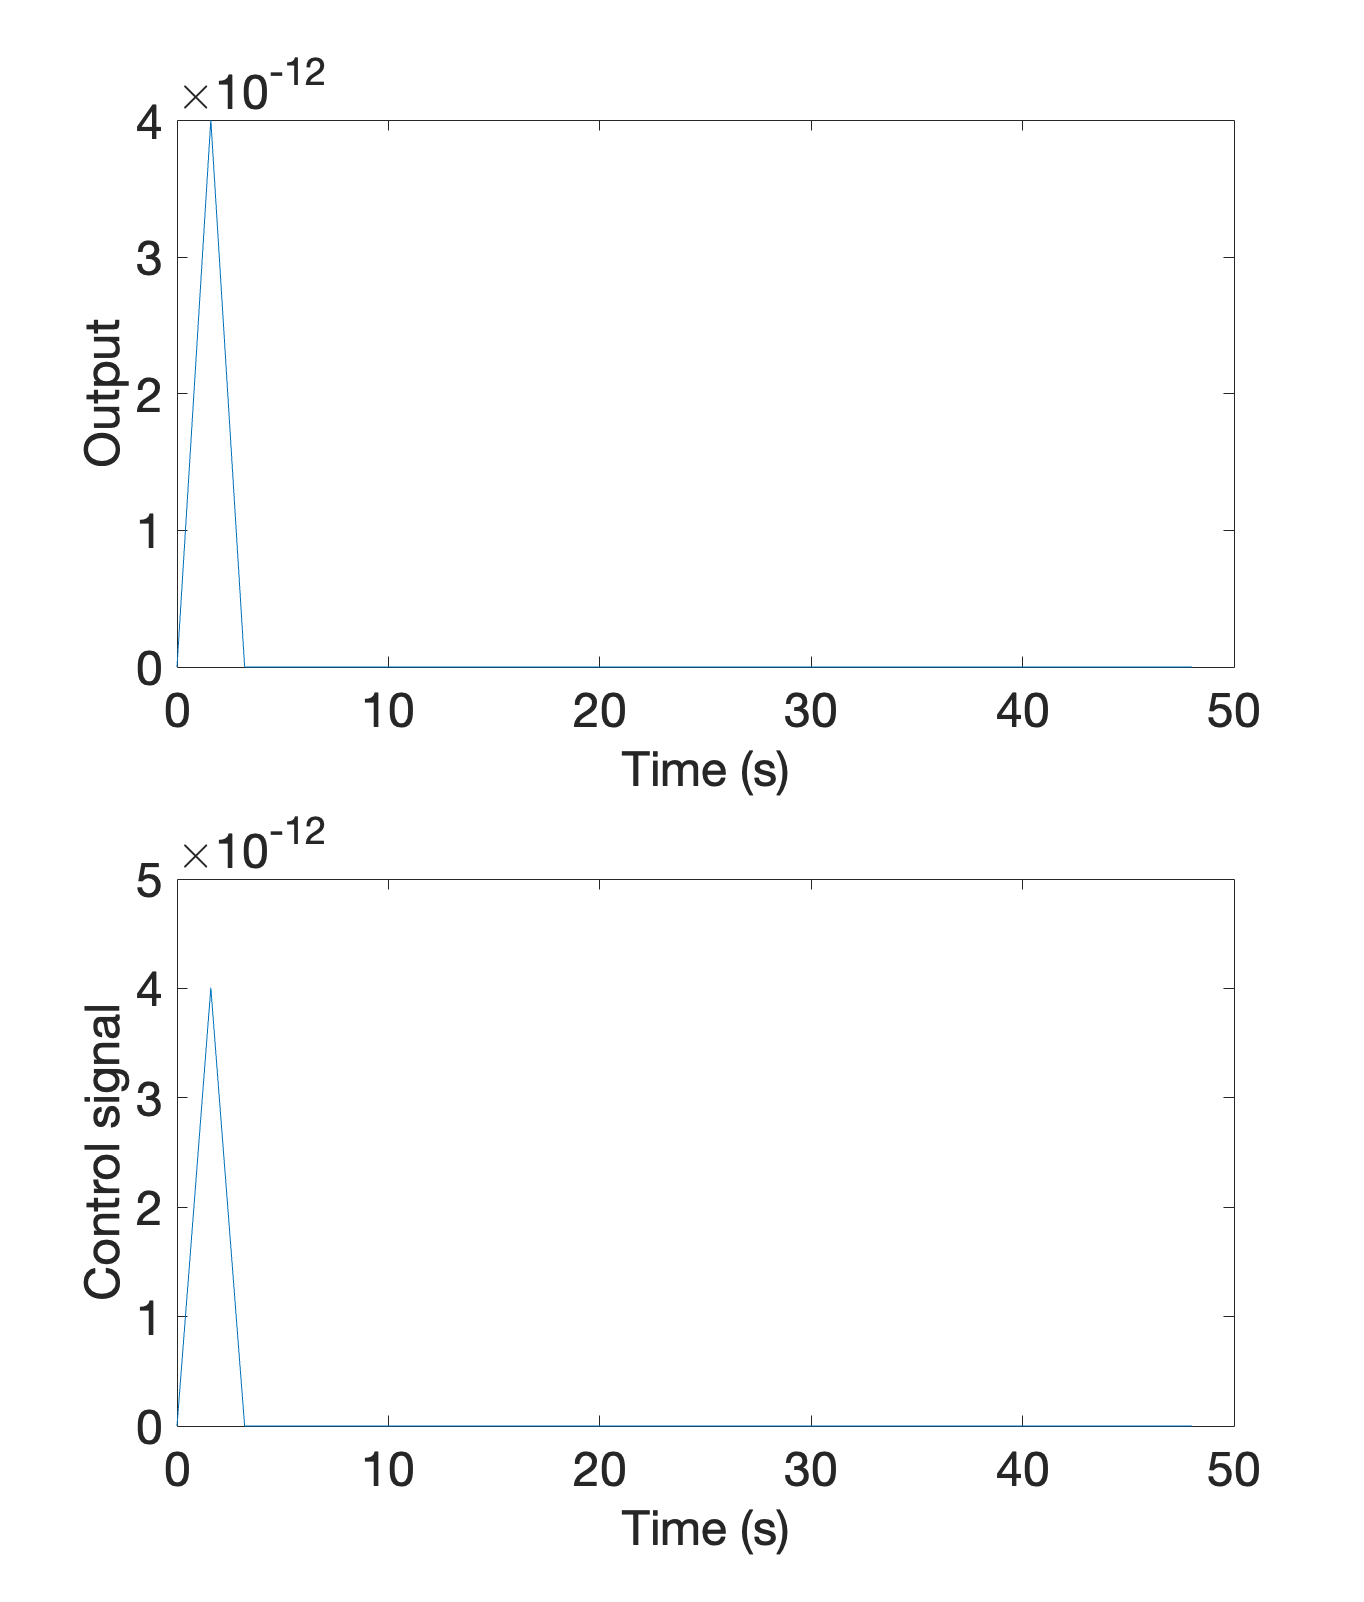
\includegraphics[width=\textwidth]{images/sstr31.png}
	\caption{Output and control of indirect adaptive implementation of minimum variance controller}
	\label{fig:sstr31}
\end{figure}

\begin{figure}
	\centering
	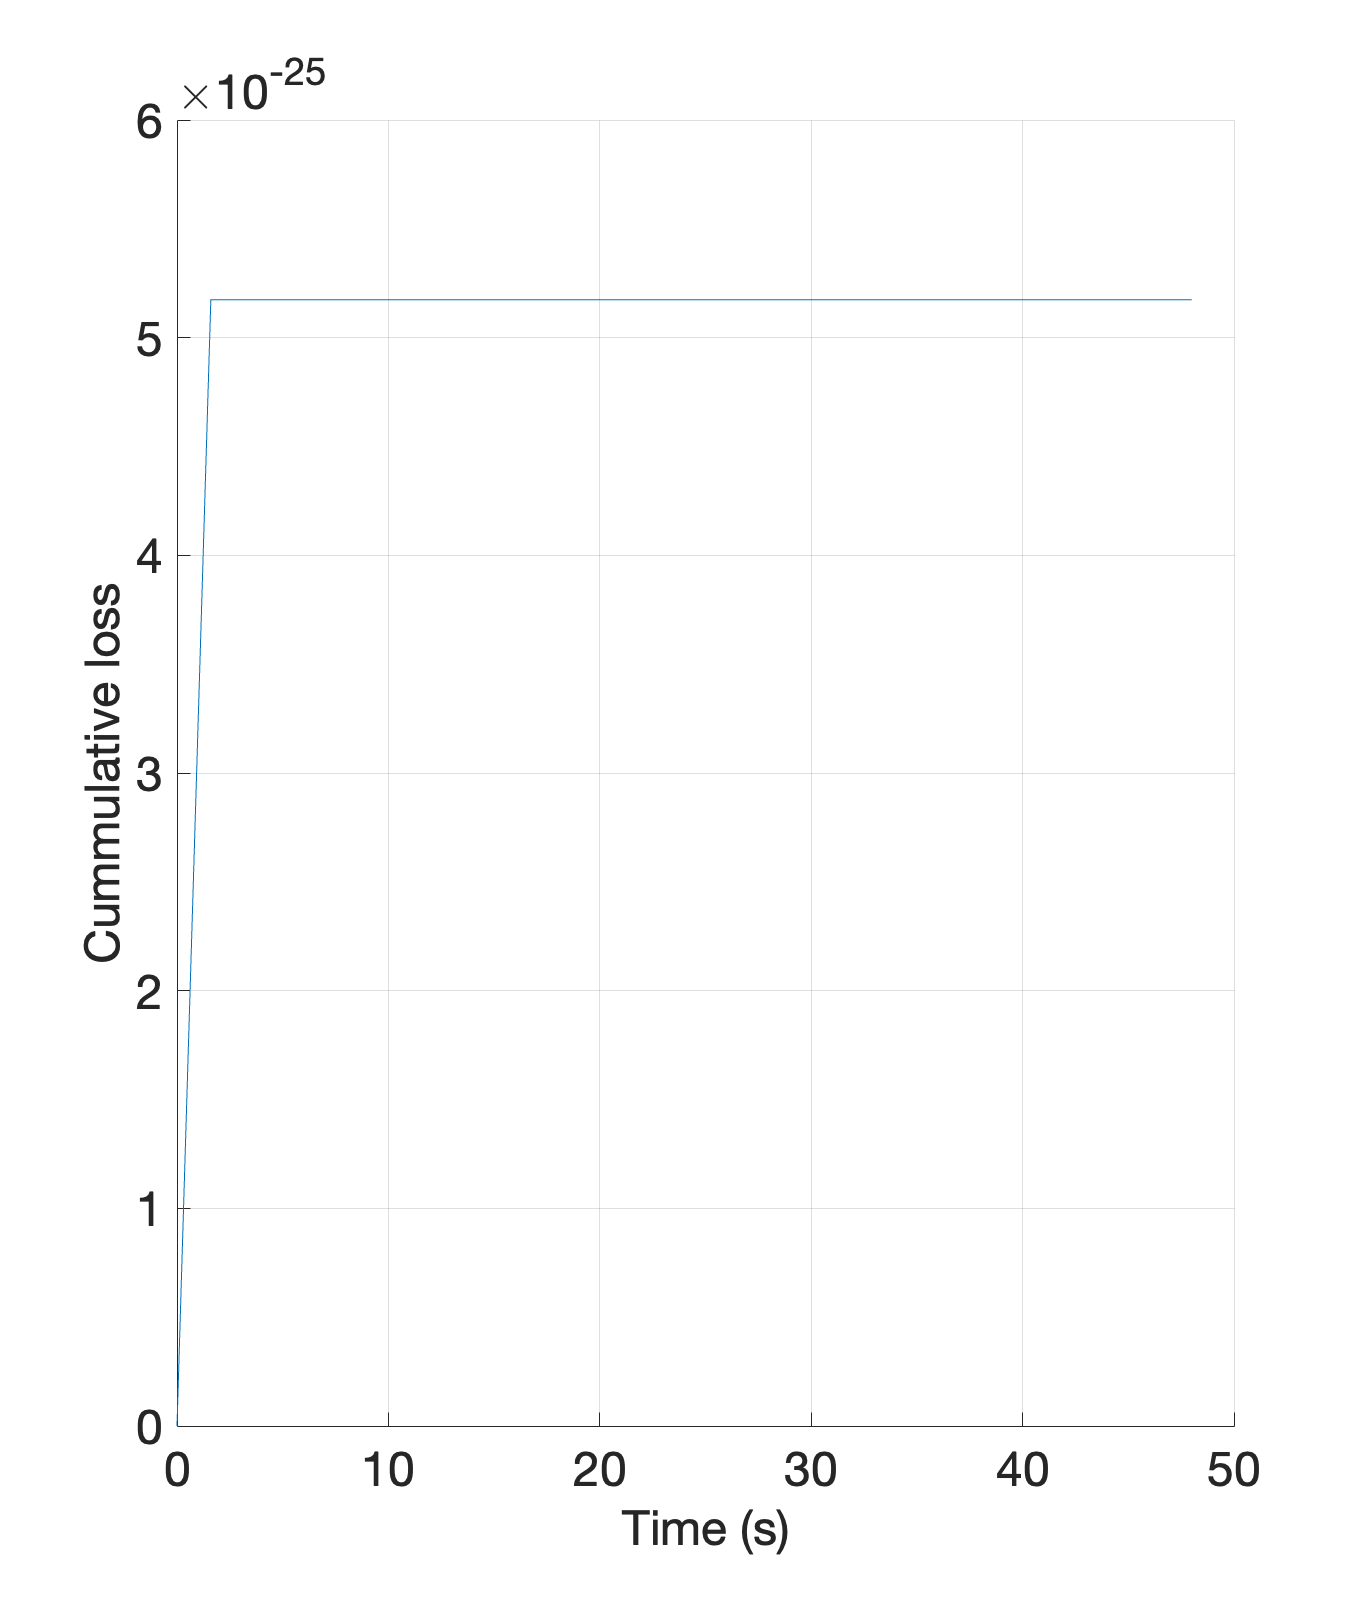
\includegraphics[width=\textwidth]{images/sstr32.png}
	\caption{Cummulative loss of indirect adaptive implementation of minimum variance controller}
	\label{fig:sstr32}
\end{figure}

\noindent The code for this section is available at \lstinline|assignment3/SSTR/SSTR_3.m|. 
